% model class
% light integration of models with relational data Vs deep integration
% UDFs: is it like a UDF or is it a UDF? Are tables with UDFs allowed to have code + data.

\section{Models}
\label{sec:models}

The proposed Plato database aims to solve the discussed problems by introducing models as first class citizens. A model is a mathematical representation of the world that predicts a quantity of interest (e.g., temperature) at every point of the spatiotemporal domain.
In the basic case, a {\em model} is a continuous function $f:\mathcal{D}\mapsto \mathcal{Q}$ from a (generally multidimensional) spatiotemporal domain $\mathcal{D}$ to $\mathcal{Q}$. In this work we consider domains $\mathcal{D}$ that are subspaces of the four-dimensional spatiotemporal domain (that includes the three space dimensions X, Y, Z and the temporal dimension T). For instance, the domain of a model can be a sphere of $(x, y, t)$ points around a center $(x_0, y_0, t_0)$, a square of $(x, y)$ points, etc.

\vspace*{0.5cm}
\begin{example}
For instance, a model for temperature may be a function $f:D_{t\_2012\_now}\mapsto Q_{float}$, which given a point in time $t$ between 2012 and now returns a float, corresponding to the \emph{predicted} temperature at time $t$.
\end{example}
\vspace*{0.5cm}

\section{Plato: An extensible model-aware database}
\label{sec:architecture}

\begin{figure}
\center
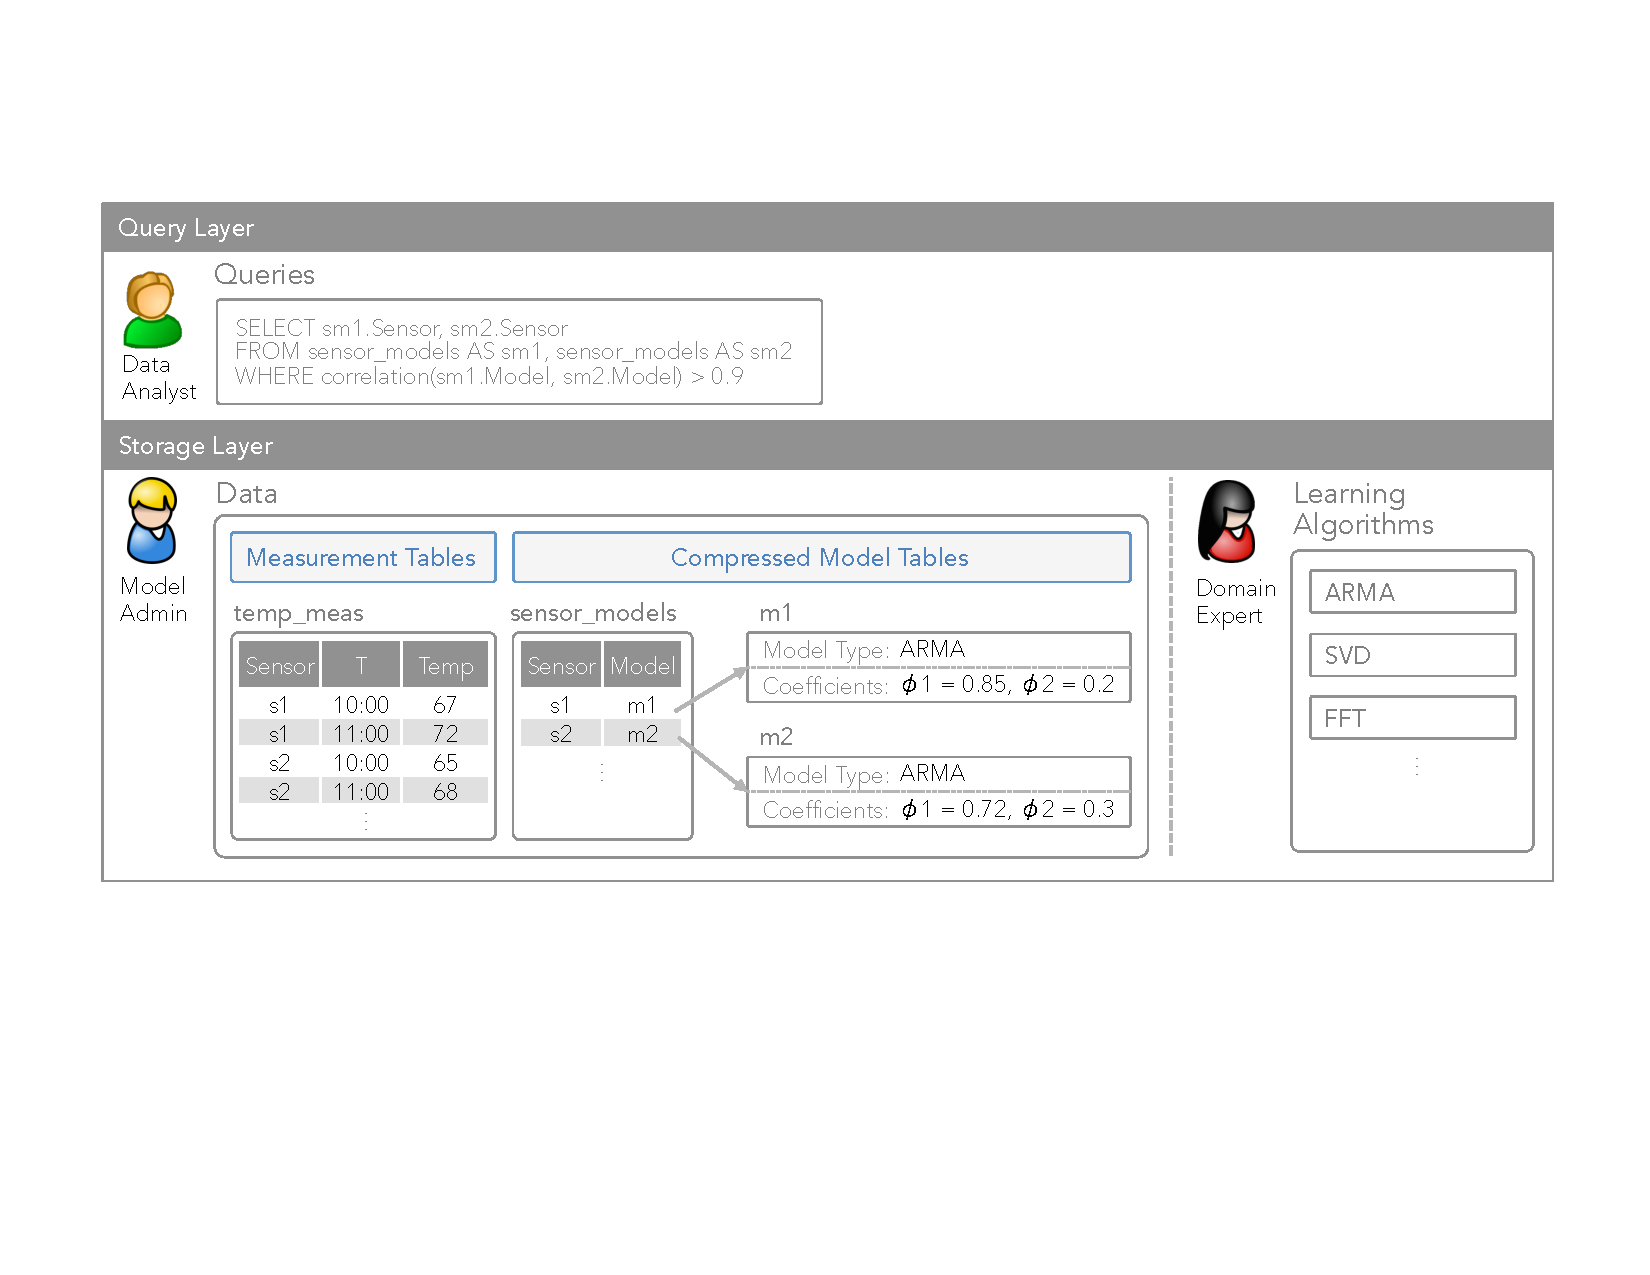
\includegraphics[width=\textwidth]{fig-architecture.pdf}
\caption{Plato Architecture}
\label{fig:basic-architecture}
\vspace*{-0.5cm}
\end{figure}

Platon facilitates the integration of models in a general database system through the architecture shown in Figure~\ref{fig:basic-architecture} and discussed next.

Raw sensor data measurements are stored in conventional SQL tables, which we refer to as {\em measurements tables}. Every measurements table contains among others a subset of the spatiotemporal attributes $X$, $Y$, $Z$ and $T$ (representing the three spatial dimensions and the temporal dimension, respectively).

\vspace*{0.5cm}
\begin{example}
Consider a measurements table with schema \texttt{temp\_meas(Sensor, T, Temp)} containing tuples of the form $(s, t, m)$, denoting that temperature sensor $s$ provided at time $t$ the temperature measurement $m$.
Attribute \texttt{Sensor} is a foreign key to another table \texttt{temp\_sensor(ID, X, Y, Installed\_on, $\ldots$)} providing the properties of each sensor, including among others its latitude and longitude.
\footnote{The data administrator can decide what is the best schema for the measurements data. For example, instead of a single table carrying all the temperature sensor measurements, the administrator may choose one table for each sensor.
}
\end{example}
\vspace*{0.5cm}

To facilitate easy data analysis, the model administrator can build models on top of the raw measurements. To generate a model, the model administrator can utilize {\em learning algorithms}, which take as input the measurements and potentially background knowledge about the real world and return a model. Learning algorithms are designed by domain specialists, who have knowledge of the domain and the underlying physical properties of the sensor data. For instance, weather experts can design a weather learning algorithm. Although some of the learning algorithms will be domain specific (such as the weather example above), others are general algorithms proposed in the machine learning literature \reminder{Yoav, can you please add a reference?} and shown to be applicable to a wide range of domains. This includes among others algorithms for learning an ARMA (Autoregressive-moving-average) model (which is suitable for readings from sensors measuring natural phenomena, such as temperature), an SVD (Singular Value Decomposition) model etc. To bootstrap the system and facilitate the quick generation of models for many common use cases, Plato comes preloaded with several such learning algorithms.

A learning algorithm $g$ has the general form of $g(R;p)$, taking as input a measurements table $R$ and a tuple $\bar{p}$ of parameter values. Since a learning algorithm should be adaptable to different scenarios (e.g., to domains of different dimensionality), it is in general polymorphic by accepting a parameter vector $p$ of variable length.

\vspace*{0.5cm}
\begin{example}
For instance, the learning algorithm $arma(R;{\bar{A}_{cont}}; \bar{A}_{meas})$ takes as input a measurements table $R$ together with the sets $\bar{A}_{cont}$, $\bar{A}_{meas}$ of attributes of $R$ that correspond to the spatiotemporal attributes and measurement attributes of $R$, respectively and creates an ARMA model $f:\mathcal{D}\mapsto\mathcal{Q}$, where $\mathcal{D}$ is the subspace of the spatiotemporal domain defined by attributes $\bar{A}_{cont}$ and $\mathcal{Q}$ is the equal to $Q_1 \times Q_2 \ldots \times Q_n$, where $Q_i$ the domain of the $i$-th attribute in $\bar{A}_{meas}$.
\end{example}  
\vspace*{0.5cm}

Models created through learning algorithms can be used as values in tables. To this end, Plato extends SQL's data types (e.g., string, integer, etc.), with a new {\em model data type} that comes with an associated model signature $\mathcal{D}\mapsto \mathcal{Q}$. An attribute of such a type is called a {\em model attribute} and accepts as values models conforming to the corresponding function signature. We will refer to a table that contains at least one model attribute as a {\em model table}. Model tables are defined by SQL view definitions that involve {\em learning algorithm} invocations. 

\vspace*{0.5cm}
\begin{example}
\label{xmpl:models-and-definitions}
For instance, in order to create a model table, containing sensor IDs and an ARMA model, representing the predicted temperatures for the particular sensor, one can write the following statement:

\begin{verbatim}
CREATE MATERIALIZED VIEW sensor_models AS 
SELECT Sensor, arma(G; T; Temp) AS Model
FROM temp_meas GROUP BY Sensor AS G(T, Temp)
\end{verbatim}

Note that for ease of exposition, we use an extension of SQL that allows the generation of nested relational tables.\footnote{Extending SQL to nested tables has been a well-studied topic in the database management field and recently it is featured in multiple ``Big Data" databases that feature semistructured models. 
}
In particular the GROUP BY operator creates for each sensor appearing the the measurements table \texttt{temp\_meas} a nested table $G$ containing all measurements for the particular sensor. These measurements are given as input to the ARMA learning algorithm to create the corresponding ARMA model.
The resulting model table \texttt{sensor\_models(Sensor, Model)} contains tuples of the form $(s, f)$, where $s$ is a sensor and $f$ the corresponding temperature ARMA model.
\end{example}
\vspace*{0.5cm}

A model table may be virtual in the sense that SQL view definitions are virtual, i.e., no actual computation is performed until a query uses them. However, in practice, the administrator is motivated to materialize models (and the  respective model tables) in order to benefit from the data compression that models enable. This can be achieved by adding the MATERIALIZED keyword in the view definition as shown above.

Note, that the administrator has in general to choose in general between multiple model algorithms, which come with different compression levels and corresponding guarantees regarding information preservation. Indeed, a major research issue, discussed in Section~\ref{sec:compression}, is the semiautomation of the choice of model algorithms, which should take into consideration the query/analytics workload.

\vspace*{0.5cm}
\begin{example}
In a modification of the running example, the administrator can choose to capture temperature in a single model \texttt{full\_model} that predicts the temperature based on \texttt{x}, \texttt{y} and \texttt{t} and is defined as follows:
\begin{verbatim}
CREATE MATERIALIZED VIEW full_model AS 
arma(SELECT X, Y, T, Temp
FROM temp_meas, temp_sensor WHERE Sensor = ID; X, Y, T; Temp)
\end{verbatim}

The reasons for doing so could be: (a) The individual sensor models may be heavily correlated based on the \texttt{X} and \texttt{Y} sensor coordinates. In such case, a single model can have a much more compact representation than the collection of individual sensor models.
(b) The analytics may need temperature predictions for specific locations, which do not coincide with any individual sensor.
\end{example}
\vspace*{0.5cm}

%\paragraph{Vector quantities} In the general case, a model's quantity is a vector (rather than a scalar) from the domain $\mathcal{\bar{Q}}$.

\paragraph{Probabilistic models} For ease of exposition, models have been defined above as returning absolute values. However, since they are inherently approximations of the underlying signal, models return in reality probability distributions of the quantities, rather than absolute values. Therefore a model is a function $f:\mathcal{D}\mapsto \mathcal{H_{Q}}$, where $\mathcal{H_{Q}}$ is the space of probability distributions over the quantity domain $\mathcal{Q}$. The probability distributions capture the certainty of the predicted values. For example, the model of Example~\ref{xmpl:models-and-definitions} can easily benefit from returning probability distributions of the predicted temperatures. A common way of displaying the probability distribution of a quantity to the end user is through a triple $(p, v, \epsilon)$, denoting that the the quantity's value falls within the interval $[v - \epsilon, v + \epsilon]$ with probability $p$.\\

%\paragraph{Viewing models as infinitely-sized tables} Notice that a model $f:\mathcal{\bar{D}}\mapsto \mathcal{H_{\bar{Q}}}$ can be also perceived as a table $R_f(\bar{D}, \bar{Q}, H)$, where the table has an infinite number of tuples, the coordinates $\bar{D}$ form a key and the attribute $H$ provides the value of the probability distribution at the specific coordinates.
%Correspondingly, the models that are the values of a table's attribute can be perceived as infinite size nested tables.%

%\paragraph{Model representations} 
%Models are associated with {\em representations}, which contain the data needed to compute the functions. For example, the representation of a model generated by Fourier analysis will consist of the significant frequencies present in the signal, possibly along with data that modulate the noise. 

\subsection{Queries and Optimized Query Evaluation}
\label{sec:queries}

\reminder{To Yannis P: The query language described below does not yet provide support for probabilities. Do we want to add it in?}
A key success factor of database systems has been the declarative SQL query language where the user/developer expresses the desired result of his analysis without having to specify the algorithm that computes this result and without having to refer to the data structures where the data are stored. The database discovers the optimal plan to compute the result, making best use of the available data structures. 

In the spirit of declarative programming, Plato offers an extension of SQL that enables declarative querying of model tables. A data analyst can query model tables in two different ways. \reminder{To YP: Please check motivation for the two methods of querying model tables and revise if needed}\\

\paragraph{Querying models through functions} According to the first approach, a SQL query over the model tables can operate on model attributes through special functions that take as input one or more models and return a scalar, a tuple, or a new model. For instance, a correlation function takes as input two models $M1$ and $M2$ and returns a scalar corresponding to their correlation. Similarly, a multiplication function takes as input a model $M$ and a scalar $c$ and returns a new model whose values are the values $M$ multiplied by $c$. Plato supports many common such functions, while additional functions can be added through a suitable API.

\vspace*{0.5cm}
\begin{example}
The function $correlation(M1, M2)$ takes as input two models $M1$ and $M2$ and computes their correlation. Continuing our running example, one can utilize this function to compute all pairs of temperature sensors whose models have a strong (i.e., greater than 0.9) correlation as follows:
\begin{verbatim}
SELECT sm1.Sensor, sm2.Sensor
FROM sensor_models AS sm1, sensor_models AS sm2
WHERE correlation(sm1.Model, sm2.Model) > 0.9
\end{verbatim}
\end{example}
\vspace*{0.5cm}

The data analyst may compose these functions to create more complex queries, as long as the top-level function that appears in the query's SELECT or WHERE clause returns a scalar or a tuple (since SQL cannot interpret model attributes). However, function composition can prevent the system from applying certain optimizations, since the query imposes a certain order of execution. For instance, specifying a three-way join through function composition imposes a certain (non-optimal) join ordering. 

\paragraph{Querying models by considering them as infinite tables} To address this issue, Plato allows data analysts to also query model tables by considering models as infinite tables on which they can execute regular SQL queries. In particular, a model $f: \mathcal{D} \mapsto \mathcal{Q}$ from vector $(x, y, z, t)$ to vector $(q_1, q_2, \ldots q_n)$ can be seen as a table of schema $f(X, Y, Z, T, Q_1, Q_2, \ldots, Q_n)$, where $(X, Y, Z, T)$ is a primary key. Conceptually this table is an infinite table containing a tuple predicting the value of the quantities $Q_1, Q_2, \ldots, Q_n$ for each value in $\mathcal{D}$.

\vspace*{0.5cm}
\begin{example}
\label{xmpl:query-infinite-tables}
For instance, each ARMA model in our running example can be seen as a table over schema (T, Temp). Thus the model table \texttt{sensor\_models} defined above is a table over schema $sensor\_models(sensor, (T, Temp))$, where $(T, Temp)$ is the schema of the nested table corresponding to the model. Using this representation, we can ask for the temperature of all sensors at midnight of 01/01/2014 through the following query:

\begin{verbatim}
SELECT sm1.Sensor, m1.Temp
FROM sensor_models AS sm1, sm1.Model AS m1
WHERE T = 2014/01/01#00:00:00
\end{verbatim}
\end{example}
\vspace*{0.5cm}

Allowing data analysts to write SQL queries over infinite tables enables Plato to perform query optimizations, such as join reordering. However, the fact that models are conceptually infinite tables also creates two major challenges:\\

\emph{(a) Defining a class of safe queries.} Since infinite tables cannot be represented in practice, Plato should only accept {\em safe queries}; i.e., queries that are guaranteed to return a finite result. Examples of such queries are queries asking about a particular point in the spatiotemporal domain, or a finite set of points. The goal of this work is to find the most general class of queries that are guaranteed to be safe.\\

\emph{(b) Defining the query answering semantics for aggregate queries.} The semantics of safe Select-Project-Join queries is well-defined, as the query is operating on the finite domain, specified by the condition that makes the query safe. For instance, in Example \ref{xmpl:query-infinite-tables} the query is not operating on the infinite spatiotemporal domain, but only on a finite domain, consisting of the single time point 2014/01/01\#00:00:00 specified in the WHERE clause. However, this does not hold for aggregate queries. Even though an aggregate query may be safe (i.e., its final result will be finite), the aggregate function may still operate on the infinite spatiotemporal domain and thus cannot be defined in the same way as in SQL. For instance, consider a model providing precipitation values and the aggregate query computing the sum of precipitation values over a week. While the SUM function is defined in SQL as the sum of a finite number of values, in the case of the model it has to be defined as the integral of the precipitation model. The goal of this work is to formally define the semantics of safe aggregate queries through the use of calculus.\\

\paragraph{Probabilistic queries} Since models return probability distributions, any query can also specify probability guarantees by providing the desired probability $p$ of the result being correct. In that case, Plato returns not only a single value $v$ but a confidence interval $[v-\epsilon, v+\epsilon]$ that is guaranteed to contain the correct answer with probability $p$. Such a query can be specified through the WITH PROBABILITY clause, as illustrated through the following example.

\vspace*{0.5cm}
\begin{example}
Query of Example \ref{xmpl:query-infinite-tables} can be augmented with a guideline for returning results with 0.95 probability as follows:

\begin{verbatim}
SELECT sm1.Sensor, m1.Temp
FROM sensor_models AS sm1, sm1.Model AS m1
WHERE T = 2014/01/01#00:00:00
WITH PROBABILITY 0.95
\end{verbatim}
\end{example}
\vspace*{0.5cm}

%Unlike conventional query optimization, where the rewritings produce equivalent expressions, opportune rewritings in model-based databases are not guaranteed to produce queries with identical results. Rather, in many important cases the results are guaranteed to be equivalent under common assumptions of statistical signal processing. In other cases, they are guaranteed to be equivalent within certain error bounds. Plato queries allow the user to specify the requested guarantee by providing appropriate parameters.

%The first category utilizes various functions that input models and output statistic measures or models. The second category allows variables that range over the infinitely-many coordinate points. 


